\documentclass[amsmath,secnumarabic,floatfix,amssymb,nofootinbib,nobibnotes,letterpaper,11pt,tightenlines,showkeys]{revtex4}

\usepackage{times}

\usepackage{geometry}
\usepackage{amssymb}
\usepackage{latexsym, amsmath, amscd,amsthm}
\usepackage{graphicx}
\usepackage{array}
\usepackage[percent]{overpic}
%\usepackage{pdfsync}
\usepackage{units}
\usepackage{hyperref}
\PassOptionsToPackage{caption=false}{subfig}
\usepackage[lofdepth]{subfig}

\usepackage{clrscode}

\def\figdir{figs/}
\graphicspath{\figdir}

\newtheorem{theorem}{Theorem}
\newtheorem*{maintheorem}{Main Theorem}
\newtheorem{lemma}[theorem]{Lemma}
\newtheorem{proposition}[theorem]{Proposition}
\newtheorem{corollary}[theorem]{Corollary}

\theoremstyle{definition}
\newtheorem{definition}[theorem]{Definition}
\newtheorem*{example}{Example}
\newtheorem{conjecture}[theorem]{Conjecture}
\newtheorem{remark}[theorem]{Remark}

\def\defn#1{Definition~\ref{def:#1}}
\def\thm#1{Theorem~\ref{thm:#1}}
\def\lem#1{Lemma~\ref{lem:#1}}
\def\figr#1{Figure~\ref{fig:#1}}
\def\prop#1{Proposition~\ref{prop:#1}}
\def\cor#1{Corollary~\ref{cor:#1}}
\def\sect#1{Section~\ref{sect:#1}}
\def\mainthm#1{Main Theorem~\ref{mainthm:#1}}
\def\mainthm#1{Main Theorem~\ref{mainthm:#1}}
\def\rmark#1{Remark~\ref{rmark:#1}}
%\numberwithin{equation}{section}

% make a small change

\newcommand{\abs}[1]{\lvert#1\rvert}
\newcommand{\tvnorm}[1]{\left| #1 \right|_{\operatorname{TV}}}
\newcommand{\R}{\mathbb{R}}
\newcommand{\C}{\mathbb{C}}
\newcommand{\Q}{\mathbb{H}}
\newcommand{\Z}{\mathbb{Z}}
\newcommand{\F}{\mathbb{F}}

\newcommand{\arc}[1]{\gamma_{#1}}
\newcommand{\len}[1]{\ell_{#1}}
\newcommand{\bdry}{\partial}
\newcommand{\bdy}{\bdry}
\newcommand{\isom}{\cong}
\newcommand{\setm}{\smallsetminus}
\newcommand{\eps}{\varepsilon}
\newcommand{\lk}{\textrm{lk}}
\newcommand{\intr}{\textrm{int}} %interior
\newcommand{\half}{\tfrac12}
\newcommand{\arcsec}{\textrm{arcsec}}
\newcommand{\m}{\mathcal}
\renewcommand{\d}{\partial}
\newcommand{\grad}{\nabla}
\newcommand{\PThree}{\ePol_3(n)/\SO(3)}
\newcommand{\EOne}{E_1}
\newcommand{\ETwo}{E_2}
\newcommand{\FOne}{F_1}

\newcommand{\loopinsert}{E_1}
\newcommand{\edgedouble}{E_2}
\newcommand{\cutedgedouble}{E_3}
\newcommand{\pairinsert}{E_4}
\newcommand{\plantri}{\texttt{plantri} }
\newcommand{\nauty}{\texttt{nauty} }
\newcommand{\saucy}{\texttt{saucy} }


\graphicspath{{../../figs/}{figs/}}

\newcommand{\eightgraph}{\raisebox{-0.17\baselineskip}{\includegraphics[height=0.81\baselineskip]{eightgraph}}}
\newcommand{\hopfgraph}{\raisebox{-0.17\baselineskip}{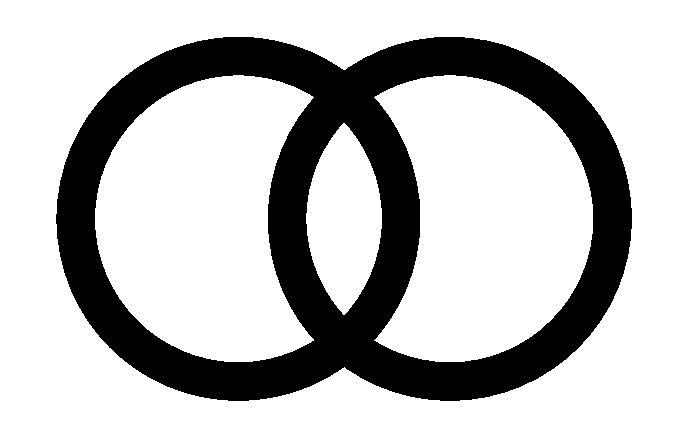
\includegraphics[height=0.81\baselineskip]{hopfgraph}}}


\bibliographystyle{plain}
%
\def\co{\colon\!}

\setlength{\parskip}{5pt}

\let\mgp=\marginpar \marginparwidth18mm \marginparsep1mm
\def\marginpar#1{\mgp{\raggedright\tiny #1}}
%\def\marginpar#1{}   %Uncomment this to hide all marginpars

\let\lbl=\label
\def\label#1{\lbl{#1}\ifinner\else\marginpar{\ref{#1} #1}\ignorespaces\fi}

\bibliographystyle{plain}

\begin{document}
\title[]{Knot Probabilities in Random Diagrams}
\author{Jason Cantarella, Harrison Chapman, Eric Lybrand, Hollis Neel and Malik Henry}
\altaffiliation{University of Georgia, Mathematics Department, Athens GA}
\noaffiliation
\author{Matt Mastin}
\altaffiliation{Wake Forest University, Mathematics Department, Athens GA}
\noaffiliation
\author{Eric Rawdon(?)}
\altaffiliation{Wake Forest University, Mathematics Department, Athens GA}
\noaffiliation

\maketitle

Suppose that one is given an $n$-crossing knot diagram chosen at random from the (finite) set of such diagrams. What is the probability that it is a diagram of the unknot? In this paper, we report on a computer experiment which gives precise answers to this and similar questions for $n \leq 12$ by direct enumeration and classification of knot diagrams. From the point of view of classical knot theory, this is a particularly simple model of random knotting. Part of our interest is to provide data which can be compared to results about more complicated distributions, such as the distribution of knots provided by selecting random closed equilateral $n$-gons, closed lattice walks, or in combinatorial models such as Even-Zohar et.\ al.\'s \emph{Petaluma} model.

\section{Definitions}

We begin with some definitions
\begin{definition}
We define a \emph{link shadow} with $n$ vertices to be an equivalence class of connected $4$-regular embedded planar multigraphs with $n$ vertices up to \emph{shadow isomorphism} which is a graph isomorphism which preserves the counterclockwise order of edges around each vertex.
\end{definition}

Examples of link shadows are shown below
\begin{center}
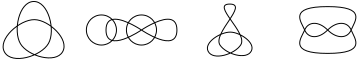
\includegraphics[width=4in]{linkshadow}
\end{center}
It is well-understood that the equivalence relation preserves the (spherical) embedding of the planar graph; in fact, the left and right-most shadows are actually equivalent under embedded isomorphism-- we have just changed the ``exterior'' face of the projection from the sphere to the plane. 

We can partition the edges of a link diagram into \emph{components} by defining two edges to be equivalent if they meet at a vertex at positions which are not cyclicly adjacent. We will call shadows with a single component \emph{knot shadows}. They will be the focus of this paper. 

It's standard in knot theory that
\begin{proposition}
The finite set of knot shadows with $n$ vertices is bijective to the finite set of generic immersions of $S^1$ into $S^2$ up to orientation-preserving diffeomorphism of the sphere.
\end{proposition}

We can define a link diagram by 
\begin{definition}
A \emph{link diagram} is a link shadow where each component is oriented and each vertex is decorated with over-under information for the edges meeting at the vertex. We call these vertices \emph{crossings}. The equivalence relation for these diagrams is the \emph{diagram automorphism}: a shadow isomorphism which also preserves orientation and over-under information. 
\end{definition}
It is clear that there are at most $2^{\text{\# components}} 2^{\text{\# crossings}}$ link diagrams associated to a given link shadow, but that this number may be reduced if there are nontrivial diagram automorphisms.

Various models of random knots have been proposed in the literature. In this paper, we will examine a quite natural one: 
\begin{definition}
In the \emph{random diagram model}, a random $n$-crossing knot is selected uniformly from the counting measure on the finite set of one-component $n$-crossing link diagrams.
\end{definition}
We intend to compute knot probabilities directly in the random diagram model for (relatively) small $n$ by direct enumeration of the collection of $n$-crossing random knots. Having the entire collection of diagrams will in addition allow us to study transitions between diagrams, but we will discuss this in future work. 

\section{Constructing the database of diagrams}

Our first goal is to enumerate the link shadows-- that is, the connected 4-regular embedded planar (multi)graphs-- computationally.  The basic strategy for such an enumeration is to define a smaller class of graphs so that the graphs we are interested in can be obtained from the base class of graphs by various expansion moves. Lehel~\cite{JGT:JGT3190050412} gave a strategy for generating all 4-regular graphs in this way from the octahedral graph. Instead of using Lehel's strategy directly, we build on the method of Brinkmann and McKay~\cite{Brinkmann:2007up,McKay:1998wa} for enumerating isomorph-free embedded planar graphs; we extend their work here to generate the class of graphs that we're interested in. We note that if we were only interested in 4-edge-connected diagrams (that is, prime diagrams), we could generate them as the duals of the planar simple quadrangulations generated by \plantri following~\cite{Brinkmann:2005um}. But since we are interested in all the diagrams, this approach is not immediately\footnote{We could generate all prime diagrams and connect-sum them to generate the composite ones, but the bookkeeping becomes intricate quickly and it's not easy to debug.} open to us.

In the spirit of Brinkmann and McKay, we now define four expansion moves of embedded planar graphs with vertex degree $\leq 4$ which generate new embedded planar graphs of vertex degree $\leq 4$ with the same number of vertices, but additional edges:
\begin{definition}
The four expansion operations that we will use are the following:
\begin{itemize}
\item $\loopinsert$ Loop insertion adds a loop edge to a vertex of degree 1 or 2, as below.\\
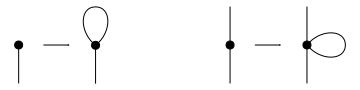
\includegraphics[width=4in]{loop-addition.png}
\item $\edgedouble$ bigon-creation edge doubling duplicates an existing edge joining vertices of degree $< 4$ so as to create a new bigon face, as below.\\
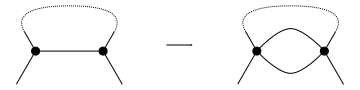
\includegraphics[width=4in]{edge-duplication-non-cut.png}
\item $\cutedgedouble$ cut-edge doubling also duplicates an existing edge joining vertices of degree $<4$, but requires that this edge separate the graph into two connected components. In this case, there is a different way to insert the edge which does not create a bigon with the existing edge. The operation is shown below.\\
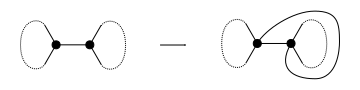
\includegraphics[width=4in]{edge-duplication-cut}
\item $\pairinsert$ pair insertion adds a pair of edges simultaneously, joining two vertices of degree 2 which are both on two faces of the embedding, as below.\\
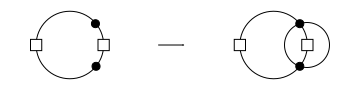
\includegraphics[width=4in]{pair-insertion}
\end{itemize}
\end{definition}

We can now show

\begin{proposition}
Every connected $4$-regular embedded planar (multi)graph $G$ can be obtained from a connected, embedded planar simple graph of vertex degree $\leq 4$ $G_0$ by a series of $\loopinsert$, $\edgedouble$, $\cutedgedouble$, and $\pairinsert$ expansions. 

Equivalently, any connected $4$-regular embedded planar (multi)graph $G$ can be reduced to a connected embedded planar simple graph $G_0$ of vertex degree $\leq 4$ by a series of $\loopinsert$, $\edgedouble$, $\cutedgedouble$, and $\pairinsert$ reductions. The embedded isomorphism type of $G_0$ is determined by the  embedded isomorphism type of $G$ (the order in which the reductions are performed doesn't matter). 
\label{prop:reduce}
\end{proposition}

An illustration of the process we describe is 
\begin{center}
\includegraphics[width=4in]{expansion-from-simple-graph}
\end{center}

\begin{proof} 
We will prove the second statement, reducing in stages from some $G_n = G$ to $G_0$ by performing one reduction at each step. The number of steps we can perform is clearly finite, since each reduces the number of edges by at least one. So suppose we are at stage $G_i$. If there are no loop or multiple edges, we're done, and this is the simple graph $G_0$. 

If there is a loop edge, we can remove it with a $\loopinsert$ move. If there is a multiple edge, we must consider several cases. We can think of each vertex of $G_i$ as retaining a list of 4 connection points, ordered counterclockwise, from the initial embedding of $G$. Since we have performed some reductions already, some of these may be empty, but at least two are filled at each end of the multiple edge. Pick one vertex of the multiple edge and call it $v$ and the other vertex $w$.

If the edge multiplicity is four, $G$ is \hopfgraph. This is obtained from the graph with one edge and two vertices by two $\edgedouble$ moves. If the edge multiplicity is three or two, there is more work to do.

So there is at least one connection point on $v$ which is not occupied by a copy of the multiple edge followed immediately by a connection point which is occupied by a copy $e$ of the multiple edge. Without loss of generality, we'll call $e$ the \emph{base copy} of the multiple edge, and its connection point to at $v$ position $0$ around $v$. The remaining connection points will be numbered $1$, $2$, and $3$. By construction, the edge joined to $v$ at position $3$ (if any) is not connected to $w$. 

We can label the other end of the base copy $e$ position $a$ on the second vertex $w$, and label the other positions $b$, $c$, and $d$, again counterclockwise. If the edge multiplicity is three, only one of these positions is unoccupied by a copy of the multiple edge. Looking at the three cases (below), we can see that by parity, it must be position $b$, and the pair of copies $0a$ and $2c$ of the multiple edge can be removed by a $\pairinsert$ operation.
\begin{center}
\includegraphics[width=4in]{multiplicity-three}\\
By parity, because we came from a 4-regular embedded planar graph only the leftmost case can occur at any stage in the reduction process.
\end{center}
We have now disposed of the case where edge multiplicity is three. If edge multiplicity is two, there is one edge unaccounted for, which joins either position $1$ or $2$ on vertex $v$ to position $b$, $c$, or $d$ on vertex $w$. Therefore, there are six cases to address. We consider them in order, starting with the $1x$ configurations.

\begin{itemize}
\item 
\begin{tabular}{m{1in}m{3in}m{1in}}
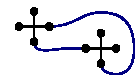
\includegraphics[width=0.9in]{1-b-configuration}
&
In the $1b$ configuration, the multiple edge forms a 2-cycle dividing the portion of the graph $G$ connected to $cd$ from the portion connected to $23$. Deleting $1b$ requires a $\cutedgedouble$ move, and the remaining base edge is a cut edge of all further-reduced $G_i$, as shown at right.
&
\includegraphics[width=0.9in]{1-b-target}
\end{tabular}
\item 
\begin{tabular}{m{1in}m{3in}}
\includegraphics[width=1in]{1-c-configuration}
&
The $1c$ configuration is forbidden by parity. 
\end{tabular}
\item 
\begin{tabular}{m{1in}m{3in}m{1in}}
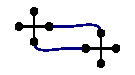
\includegraphics[width=0.9in]{1-d-configuration}
&
In the $1d$ configuration, the multiple edge forms a bigon face. Deleting $1d$ uses an $\edgedouble$ reduction, and yields the configuration at right. The remaining base edge may or may not be a cut edge of the further $G_i$.
&
\includegraphics[width=0.9in]{1-d-target}
\end{tabular}
\end{itemize}
One might think that the $2x$ configurations are simply rearrangements of those above, but this is not true. A genuinely new case arises for $2c$.
\begin{itemize}
\item 
\begin{tabular}{m{1in}m{3in}}
\includegraphics[width=0.9in]{2-b-configuration}
&
The $2b$ configuration is forbidden by parity.
\end{tabular}
\item 
\begin{tabular}{m{1in}m{3in}m{1in}}
\includegraphics[width=1in]{2-c-configuration}
&
In the $2c$ configuration, by parity, the graph $G$ must have connected $1$ and $d$ and also $3$ and $b$. None of our moves change the connectivity of the graph (because we never delete all copies of a multiple edge), so the current graph $G_i$ still joins these pairs of connection points. This means that we are in position for an $\pairinsert$ pair reduction, resulting in the graph at right.
&
\includegraphics[width=1in]{2-c-target}
\end{tabular}
\item 
\begin{tabular}{m{1in}m{3in}}
\includegraphics[width=0.9in]{2-d-configuration}
&
The $2d$ configuration is forbidden by parity.
\end{tabular}
\end{itemize}
Along the way, our analysis has been almost entirely local: we need only consider a single vertex to decide whether we can apply an $\loopinsert$ reduction and a pair of vertices to decide on $\edgedouble$, $\cutedgedouble$, and $\pairinsert$ operations. To show that order of operations doesn't matter, we need to show that whether or not we can apply these operations does not depend on which reductions have already been performed.

The three copies of a multiplicity three edge must bound two bigons, and this does not change as we reduce other edges. Therefore, the $\pairinsert$ move is always available for all multiplicity three edges.

Whether a multiplicity two edge is eligible for an $\edgedouble$ move depends only on the positions of the ends of the multiple copies on their vertices, which doesn't change as we reduce. Therefore, this operation can always be performed (or is always forbidden), regardless of which reductions have already been performed.

Whether a multiplicity two edge is eligible for a $\cutedgedouble$ or $\pairinsert$ operation depends not only on the positions of ends of edges on their vertices, but also on the connectivity of the (reduced) graph. However, as we noted above, the connectivity of the graph doesn't change as we perform reductions.

It is clear that the isomorphism type of $G_0$ does not depend on the order of reduction-- after all, in the end we are simply reducing the multiplicity of multiple edges of the edge. 

It takes only a moment longer to realize that the embedding of $G_0$ is determined as well-- this embedding is determined by the cyclic order of (surviving) edges around their vertices. We will have deleted some edges from many of these vertices by the time we reach $G_0$, potentially leaving many empty connections. However, the cyclic order of the surviving edges won't be affected by the order in which these connections were emptied. 

One might worry that the choice of \emph{which}\footnote{Remember that the choice of ``base edge'' was arbitrary.} copy of an edge of multiplicity two to delete could affect the embedded isomorphism type after an $\edgedouble$ or $\cutedgedouble$ reduction, but it's easy to check that the two possible reduced configurations are (embedded) graph isomorphic by looking at the pictures above. 
\end{proof}

We can use this theorem to come up with a strategy for generating diagrams. Basically, we will start by enumerating embedded planar simple graphs of vertex degree $\leq 4$ using \plantri, then expand them to $4$-regular embedded planar graphs using the moves above. Afterwards, we will see that we can generate embedded isomorphic graphs with different expansion sequences, so we will have to filter the graphs into isomorphism classes. We start with two lemmas:

\begin{lemma} 
If the embedded planar graph of vertex degree $\leq 4$ $G_0$ is obtained from a $4$-regular embedded planar multigraph $G$ by the reduction process of Proposition~\ref{prop:reduce} then either every vertex of degree one in $G_0$ has exactly one loop edge in $G$ and one multiedge of multiplicity two obtained by $\edgedouble$ or $\cutedgedouble$ or the graph is \hopfgraph.
\label{lem:degreeone}
\end{lemma}

\begin{proof} 
If we expand $G_0$ to $G$ using the four moves, three empty connections on the vertex must be filled during the process. If they are filled by redoubling the existing edge, then the degree of the vertex at the other end of the edge was also one, and we get \hopfgraph. Otherwise, we must fill two by adding a loop edge, and the other by doubling the existing edge. 
\end{proof}

\begin{lemma}
Two pairs of vertices $01$ and $ab$ on the unit circle may be joined by nonintersecting chords inside the circle if and only if the pairs are unlinked on the circle. That is, if $01$ and $ab$ are adjacent in the cyclic ordering of the four vertices, as opposed to an order such as $0a1b$ where the pairs alternate.
\end{lemma}

We can now design an algorithm to produce all possible expansions of $G_0$, a given connected embedded planar simple graph of vertex degree $\leq 4$ as an integer constraint satisfaction problem. By Lemma~\ref{lem:degreeone}, we must add a loop to each vertex of degree one in $G_0$ eventually. We can save time by doing so at the start of the computation. We will therefore assume that loops have been added to create a \emph{prepared} graph $G_1$, and each vertex has degree $2$, $3$, or $4$.

We will now define four classes of variables:
\begin{itemize}
\item $l_{i}$ for every vertex $v_i$ of degree $2$ 
\item $d_{i,j}$ for every edge $e_{ij}$ in the graph joining vertices of degree $<4$. 
\item $c_{i,j}$ for every $d_{i,j}$ where $e_{ij}$ is a cut edge
\item $p_{i,j}$ for every pair of vertices $v_{i}$, $v_j$ which both have degree 2 and are both on two different faces of the embedding
\end{itemize}
We take the subscripts to be unordered. That is, $d_{4,17}$ and $d_{17,4}$ are the same variable, since the edges $e_{4,17}$ and $e_{17,4}$ are the same edge.

These variables will all be valued in $0-1$, and represent the absence or presence of $\loopinsert$ loop edges, $\edgedouble$ doubles of existing edges, $\cutedgedouble$ doubles of existing cut edges, and $\pairinsert$ insertions of new pairs of edges. 

We can now define two sets of equations relating these variables.

\begin{definition}
We define the \emph{vertex degree equations} for a prepared graph $G_1$ to be the collection of equations indexed by the vertices of $G_1$ given below. For each vertex index $i$ of degree $\delta(i)$ in $G_1$
\begin{equation*}
\delta(i) + 2 l_i + \sum_j d_{i,j} + \sum_j c_{i,j} + 2 \sum_j p_{i,j} = 4
\end{equation*}
where the sums are taken over all $j$ for which the appropriate variables exist. These equations express the fact that in a complete expansion, the vertex degrees must all be four. 
\end{definition}

The pair variables $p_{i,j}$ satisfy an additional set of equations:
\begin{definition}
For each $p_{i,j}$ and $p_{k,l}$ so that the vertices $v_i, v_j, v_k$ and $v_l$ are on the same pairs of faces, we have an additional \emph{linking equation}
\begin{equation*}
p_{i,j} + p_{k,l} \leq 1
\end{equation*}
\end{definition}

These equations express the fact that the edges corresponding to a linked pair of endpoints along a face must intersect inside the face. Therefore, if two pair variables are linked, at most one of them can take the value $1$. For instance, in the situation below where there are four vertices of degree two along a pair of faces, we have six pair variables, two of which obey an additional linking equation. 
\begin{center}
\includegraphics[height=1.5in]{linked-ghost-pairs}
\end{center}
We note that in the end, at most two of the pair variables above can have value $1$, but that a number of combinations are ruled out by vertex degree equations instead of linking equations.

We have defined everything so that

\begin{proposition}
Every assignment of $\{0,1\}$ to the variables $l_i$, $d_{i,j}$, $c_{i,j}$, and $p_{i,j}$ which obeys the vertex degree equations and linking equations corresponds to a unique expansion of the prepared graph $G_1$ to a connected embedded planar $4$-regular multigraph $G$.
\end{proposition}

\begin{proof}
Actually, there is only a little to check. By the arguments in the proof of Proposition~\ref{prop:reduce}, the order of operations in a possible expansion $G_1, G_2, \dots, G_n = G$ is irrelevant. Therefore, if we can perform the indicated expansions at all, we will generate a unique $G$.

The $\loopinsert$ expansions indicated by the positive $l_i$ are always possible as long as the vertex degree at $v_i$ is small enough, which is true, because of the corresponding vertex degree equation. 

The $\edgedouble$ expansions indicated by the positive $d_{i,j}$ are always possible as long as the vertex degrees of $v_i$ and $v_j$ are small enough. This is true by their vertex degree equations.

The $\cutedgedouble$ expansions indicated by the positive $c_{i,j}$ again require small enough vertex degrees at $v_i$ and $v_j$ (which is again true by the vertex degree equations), and also require $e_{i,j}$ to be a cut edge of the current graph $G_i$. It is, because being a cut edge doesn't change as we perform our expansion moves.

This much was easy. The $\pairinsert$ expansions are a little more difficult.
Each $\pairinsert$ indicated by a positive $p_{i,j}$ requires several conditions. First, vertex degrees at $v_i$, $v_j$ must be small enough, which is checked as before by vertex degree equations. But the $v_i$ and $v_j$ must still be on two faces in the expansion $G_i$, which is not obvious, because previous $\pairinsert$ expansions have split faces of $G_1$ into smaller faces in $G_i$. Let us suppose that $v_i$ and $v_j$ were on the pair of faces $F_1$ and $F_2$ of the original graph. 
\begin{center}
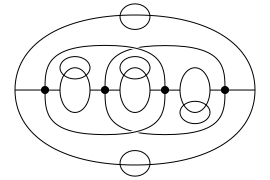
\includegraphics[width=2in]{pair-interference} 
\end{center}
The pair of faces can make contact with each in several disconnected arcs, as shown above. Further, additional pair edges can share $F_1$ or $F_2$ with some other face. However, slicing $F_1$ can only separate $v_i$ and $v_j$ if the endpoints of the splitting arc link $v_i$ and $v_j$ on $F_1$. This can't happen if the splitting arc is part of a pair which share $F_1$ with some other face (as shown), as the interfaces of $F_1$ and other faces are all connected. 

But if the splitting arc also shared $F_1$ and $F_2$, the corresponding pair variable $p_{k,l}$ is related to $p_{i,j}$ by a linking equation if and only if adding that arc would leave $v_i$ and $v_j$ on different faces. The linking equation implies that only one of the arcs indicated by $p_{i,j}$ and $p_{k,l}$ is present in the expansion; since we have assumed that $p_{i,j}$ is positive, no such $p_{k,l}$ can have already been inserted earlier in the expansion process. This concludes the case where the interface of $F_1$ and $F_2$ was disconnected.

\begin{center}
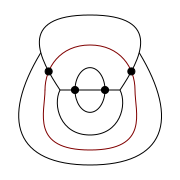
\includegraphics[width=2in]{connected-pair-interaction-case}
\end{center}

If the interface between $F_1$ and $F_2$ is connected, than either might have a disconnected interface with (at most one) other face, as shown above. This case is only cosmetically different-- again the key point is that the pair $v_i$, $v_j$ can link along the boundary of $F_1$ (or $F_2$) with a pair edge which also shares $F_1$ and $F_2$ while pairs involving a third face won't link the vertices we're interested in.
\end{proof}

We have reduced the problem to that of building and satisfying the vertex degree and linking equations. This problem is basically standard, and we use the usual branch-and-bound algorithm. We must define a canonical order on the variables (it doesn't matter how, but to be specific, in our implementation we sort the classes of variables in the order $p_{ij} \prec c_{i,j} \prec d_{i,j} \prec l_i$ and in dictionary order by the (sorted) pair $\{i,j\}$ within each class). Then we enumerate the possible assignments of $\{0,1\}$ to variables recursively, pruning the tree whenever a vertex degree or linking equation is violated. As usual, this is in theory possibly exponentially slow, but in practice quite efficient.

We now consider the problem of dividing the results into embedded isomorphism classes. We first observe that we have already shown in Proposition~\ref{prop:reduce} two different reduced graphs $G_0$ and $G_0'$ cannot expand to the same $G$ since the embedded isomorphism type of the reduction $G_0$ is determined by the embedded isomorphism type of the expansion. However, it is possible for two different collections of expansion moves for the \emph{same} graph $G_0$ to produce isomorphic $G$ and $G'$ as in the picture below:
\begin{center}
\includegraphics[width=4in]{isomorphic-expansions}
\end{center}
Therefore, we must insert each expansion we generate from a solution to the vertex degree and linking constraints into a container which rejects the solution if an embedded isomorphic graph already exists in the container. Though very fast graph isomorphism checkers such as \nauty and \saucy might speed things up, the number of vertices here is very small and we get entirely acceptable performance simply by using a hashing scheme and then attempting to build isomorphisms by pruned search.

The overall workflow is then as follows:
\begin{center}
\includegraphics[width=4in]{workflow}
\end{center}
After this, it is trivial to filter out the one-component diagrams.

\section{Classifying knot types}

homfly
mathematica
snappy

\section{Results}

giant pictures, compared with tait's classification
our distributions
monogon and bigon fractions
degree of alternatingness
universal properties? comparison with distribution from ERPs, lattice walks, and petaluma.

\section{Future Directions}

transitions, unknotting number and so forth.

\bibliography{knotprobabilitypapers}


\end{document}
